\chapter{Word2Vec \cite{nlp-1}}

\begin{enumerate}
    \item Word2vec embeddings are \textbf{static embeddings}, meaning that the method learns one fixed embedding for each word in the vocabulary.
    
    \item The intuition of word2vec is that instead of counting how often each word w occurs near, say, apricot, we’ll instead train a classifier on a binary prediction task: “Is word w likely to show up near apricot?” 
    
    \item We don’t actually care about this prediction task; instead we’ll take the learned classifier weights as the word embeddings.

    \item (\textbf{self-supervision}) The revolutionary intuition here is that we can just use running text as implicitly supervised training data for such a classifier; a word c that occurs near the target word \textbf{apricot} acts as gold ‘correct answer’ to the question “\textit{Is word c likely to show self-supervision up near apricot?}”\\
    avoids the need for any sort of hand-labeled supervision signal.

    \item word2vec is a much simpler model than the neural network language model:
    \begin{enumerate}
        \item word2vec simplifies the task (making it binary classification instead of word prediction)

        \item word2vec simplifies the architecture (training a logistic regression classifier instead of a multi-layer neural network with hidden layers that demand more sophisticated training algorithms)
    \end{enumerate}
\end{enumerate}

\section{Embedding \cite{nlp-1}}\label{Embedding}
\begin{enumerate}
    \item powerful word representation
    
    \item short \textbf{dense vectors} \indexlabel{dense vectors}\\
    instead of vector entries being sparse, mostly-zero counts or functions of counts, the values will be real-valued numbers that can be negative.

    \item embeddings are \textbf{short}, with number of dimensions $d$ ranging from $50-1000$, rather than the much larger vocabulary size $|V|$ or number of documents $D$

    \item These $d$ dimensions don’t have a clear interpretation.

    \item dense vectors work \textbf{better} in every NLP task than sparse vectors.\\
    \textbf{Intuition}: Representing words as $300$-dimensional dense vectors requires our classifiers to learn far fewer weights than if we represented words as $50,000$-dimensional vectors, and the smaller parameter space possibly helps with generalization and avoiding overfitting.

    \item Dense vectors may also do a better job of capturing \textbf{synonymy}. (SEE: \fullref{Synonymy})

    
\end{enumerate}

\subsection{Semantic properties of embeddings \cite{nlp-1}}
One parameter of vector semantic models that is relevant to both sparse tf-idf vectors (SEE: \fullref{TF-IDF: concept}) and dense word2vec vectors is the size of the context window used to collect counts. This is generally between $1$ and $10$ words on each side of the target word (for a total context of $2-20$ words).
\begin{enumerate}
    \item \textbf{Shorter context windows}
    \begin{enumerate}
        \item tend to lead to representations that are a bit more syntactic, since the information is coming from immediately nearby words.
        \item When the vectors are computed from short context windows, the most similar words to a target word $w$ tend to be semantically similar words with the same parts of speech.
    \end{enumerate}

    \item \textbf{long context windows}: When vectors are computed from long context windows, the highest cosine words to a target word w tend to be words that are topically related but not similar.

    \item Two words have \textbf{first-order co-occurrence}\indexlabel{first-order co-occurrence} (sometimes called \textbf{syntagmatic association}\indexlabel{syntagmatic association}) if they are typically nearby each other.\\
    \textbf{Example}: \textit{wrote} is a first-order associate of \textit{book} or \textit{poem}.

    \item Two words have \textbf{second-order co-occurrence} \indexlabel{second-order co-occurrence} (sometimes called \textbf{paradigmatic association}\indexlabel{paradigmatic association}) if they have similar neighbors.\\
    \textbf{Example}: \textit{wrote} is a second-order associate of words like \textit{said} or \textit{remarked}.

\end{enumerate}

\subsubsection{Analogy/ Relational Similarity \cite{nlp-1}}\label{Analogy/ Relational Similarity}
\begin{enumerate}
    \item \textbf{parallelogram model}\indexlabel{parallelogram model}: for solving simple analogy problems of the form \textit{a is to b as a* is to what?}

    \item For $\mathbf{a : b :: a^*: b^*}$ problem, meaning the algorithm is given vectors $\mathbf{a, b}$, and $\mathbf{a^*}$ and must find $\mathbf{b^*}$, the parallelogram method is thus:
    \[
        \hat{\mathbf{b}}^* = \arg\min_x distance(\mathbf{x,b-a+a^*})
    \]

    
\end{enumerate}

\subsubsection{Historical Semantics \cite{nlp-1}}\label{Embeddings: Historical Semantics}

\begin{figure}[h]
    \centering
    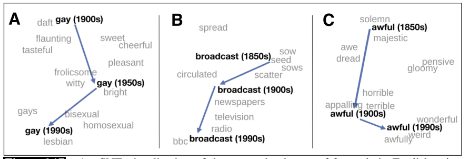
\includegraphics[width=0.6\linewidth, height=5cm, keepaspectratio]{Pictures/info-retrieval/embedding-historical-semantics.png}
    \caption{Embeddings: Historical Semantics}
\end{figure}

Embeddings can also be a useful tool for studying how meaning changes over time, by computing multiple embedding spaces, each from texts written in a particular time period.




\section{Skip-gram \cite{nlp-1}}\label{Skip-gram}
\textbf{Intuition}:
\begin{enumerate}
    \item Treat the target word and a neighboring context word as positive examples.
    \item Randomly sample other words in the lexicon to get negative samples.
    \item Use logistic regression to train a classifier to distinguish those two cases.
    \item Use the learned weights as the embeddings.
\end{enumerate}

\vspace{0.2cm}
\noindent\textbf{Note}:
\begin{enumerate}
    \item skip-gram trains a probabilistic classifier that, given a test target word $w$ and its context window of $L$ words $c_{1:L}$, assigns a probability based on how similar this context window is to the target word.

    \item The probability is based on applying the \fullref{Logistic function} to the dot product of the embeddings of the target word with each context word. 
    
    \item To compute this probability, we just need embeddings for each target word and context word in the vocabulary.
\end{enumerate}


\subsection*{Notations}
\begin{table}[h]
    \begin{minipage}{0.44\linewidth}
        \begin{figure}[H]
            \centering
            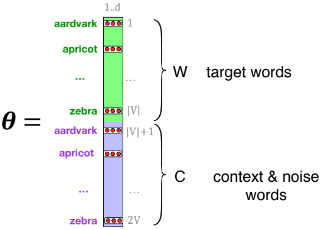
\includegraphics[width=\linewidth, height=5cm, keepaspectratio]{Pictures/info-retrieval/skip-gram-6-13.png}
        \end{figure}
    \end{minipage}
    \hfill
    \vrule
    \hfill
    \begin{minipage}{0.55\linewidth}
        \begin{figure}[H]
            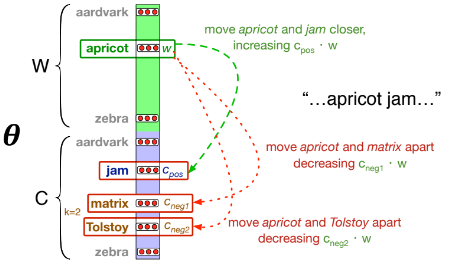
\includegraphics[width=\linewidth, height=5cm, keepaspectratio]{Pictures/info-retrieval/skip-gram-6-14.png}
        \end{figure}
    \end{minipage}
\end{table}

\begin{table}[H]
    \begin{tabular}{l l l}
        $\mathbf{W}$ & $\mathbb{R}^{|V|\times 1}$ & target words \\
        $\mathbf{C}$ & $\mathbb{R}^{|V|\times 1}$ & context \& noise words \\
        $\bm{\theta}$ & $\mathbb{R}^{2|V|\times 1}$ & \\
    \end{tabular}
\end{table}        

\subsection{Classifier - Example \cite{nlp-1}}
\begin{enumerate}
    \item Imagine a sentence like the following, with a target word apricot, and assume we’re using a window of $L = \pm 2$ context words:
    \begin{table}[h]
        \centering
        \begin{tabular}{c c c c c c c c c}
            $\cdots$ & lemon, a & \textbf{[tablespoon} & \textbf{of} & \textbf{apricot} & \textbf{jam,} & \textbf{a]} & pinch & $\cdots$ \\
             &  & c1 & c2 & w & c3 & c4 &  &  \\
        \end{tabular}
    \end{table}

    \item \textbf{Goal}: train a classifier such that, given a tuple $(w, c)$ of a target word $w$ paired with a candidate context word $c$ it will return the probability that $c$ is a real context word: \[ P(+|w, c) \]

    \item The probability that word $c$ is not a real context word for $w$ is just $1$ minus: \[ P(-|w, c) = 1-P(+|w, c) \]

    \item The \textbf{intuition} of the skip-gram model is to base this probability on embedding similarity:\\
    a word is likely to occur near the target if its embedding vector is similar to the target embedding.\\
    To compute similarity between these dense embeddings, we rely on the intuition that two vectors are similar if they have a high \textbf{dot product}
    \[ \rcmdXSimilarity(w,c) \approx \mathbf{c\cdot w} \hfill \in (-\infty,\infty) \]

    \item Using \fullref{Logistic function}:
    \[
        \displaystyle P(+|w, c) = \sigma(\mathbf{c\cdot w}) = \dfrac{1}{1 + \exp(-\mathbf{c\cdot w})} \hfill \in [0,1]
    \]
    \[
        P(-|w, c) = 1 - P(+|w, c) = \sigma(\mathbf{-c\cdot w}) = \dfrac{1}{1 + \exp(\mathbf{c\cdot w})} \hfill \in [0,1]
    \]

    \item For multiple context words in window:
    \[
        \displaystyle P(+|w, c_{1:L}) = \prod_{i=1}^{L} \sigma(\mathbf{c_i\cdot w})
    \]
    \[
        \displaystyle \log(P(+|w, c_{1:L})) = \sum_{i=1}^{L} \log(\sigma(\mathbf{c_i\cdot w}))
    \]

    
\end{enumerate}


\subsection{Learning skip-gram embeddings \cite{nlp-1}}
\begin{enumerate}
    \item \textbf{Input}: corpus of text, and a chosen vocabulary size $N$.

    \item Assign a \textbf{random embedding vector} for each of the $N$ vocabulary words, and then proceeds to iteratively shift the embedding of each word $w$ to be more like the embeddings of words that occur nearby in texts, and less like the embeddings of words that don’t occur nearby.

    \item For training a binary classifier we also need \textbf{negative examples}.
    
    \item \textbf{Skip-gram with negative sampling (SGNS)} uses more negative examples than positive examples (with the ratio between them set by a parameter $k$).

    \item For each of these $(w, c_{pos})$ training instances we’ll create $k$ negative samples $c_{neg_1},...,c_{neg_k}$, each consisting of the target $w$ plus a ‘noise word’ $c_{neg_i}$.\\
    A \textbf{noise word}\indexlabel{noise word} is a random word from the lexicon, constrained not to be the target word w.

    \item The noise words are chosen according to their \fullref{Weighted Unigram Frequency (p alpha)}, where $\alpha$ is a weight.

    \item Given the set of positive and negative training instances, and an initial set of embeddings, the goal of the learning algorithm is to adjust those embeddings to
    \begin{enumerate}
        \item Maximize the similarity of the target word, context word pairs $(w, c_{pos})$ drawn from the positive examples
        \item  Minimize the similarity of the $(w, c_{neg})$ pairs from the negative examples.
    \end{enumerate}

    \item \textbf{Loss}:
    \begin{align*}
        L_{CE} 
        &= -\log\left[ P(+|\mathbf{w, c_{pos}}) \prod_{i=1}^{k} P(-|\mathbf{w, c_{neg_i}}) \right]\\ 
        &= -\left[ \log(P(+|\mathbf{w, c_{pos}})) + \sum_{i=1}^{k} \log(P(-|\mathbf{w, c_{neg_i}})) \right]\\ 
        &= -\left[ \log(P(+|\mathbf{w, c_{pos}})) + \sum_{i=1}^{k} \log(1-P(+|\mathbf{w, c_{neg_i}})) \right]\\ 
        &= -\left[ \log(\sigma(\mathbf{c_{pos}\cdot w})) + \sum_{i=1}^{k} \log(\sigma(\mathbf{-c_{neg_i}\cdot w})) \right]\\ 
    \end{align*}
    \[
        \displaystyle \dfrac{\partial L_{CE}}{\partial c_{pos}} = [\sigma(\mathbf{c_{pos}\cdot w})-1]\cdot \mathbf{w} \hfill \displaystyle \dfrac{\partial L_{CE}}{\partial c_{neg}} = [\sigma(\mathbf{c_{neg}\cdot w})]\cdot \mathbf{w}
    \]
    \[
        \displaystyle \dfrac{\partial L_{CE}}{\partial w} = [\sigma(\mathbf{c_{pos}\cdot w})-1]\cdot \mathbf{c}_{pos} + \sum_{i=1}^{k}[\sigma(\mathbf{c_{neg_i}\cdot w})-1]\cdot \mathbf{c}_{neg_i}
    \]


    \item we want to \textbf{maximize} the dot product of the word with the actual context words, and \textbf{minimize} the dot products of the word with the k negative sampled non-neighbor words.

    
    
\end{enumerate}

\section*{Disadvantages of word2vec \cite{nlp-1}}
\begin{enumerate}
    \item \textbf{Unknown Words}: words that appear in a test corpus but were unseen in the training corpus.

    \item \textbf{word sparsity}: in languages with rich morphology, where some of the many forms for each noun and verb may only occur rarely.
\end{enumerate}

\section{Fasttext \cite{nlp-1}}\label{Fasttext}
SEE: \url{https://fasttext.cc}

\vspace{0.2cm}
\noindent Uses \textbf{subword} models, representing each word as itself plus a bag of constituent n-grams, with special boundary symbols \texttt{<} and \texttt{>} added to each word.

\vspace{0.2cm}
\noindent\textbf{Example}:\\
\begin{enumerate}
    \item $n=3$
    \item \textbf{word}: where
    \item \textbf{embeddings}: \\ \texttt{<where>} \\ \texttt{<wh, whe, her, ere, re>}
\end{enumerate}

\begin{enumerate}
    \item Then a skipgram embedding is learned for each constituent n-gram, and the word where is represented by the sum of all of the embeddings of its constituent n-grams.
    
    \item Unknown words can then be presented only by the sum of the constituent n-grams.
\end{enumerate}



\section{Global Vectors (GloVe) \cite{nlp-1}}\label{Global Vectors (GloVe)}

\begin{enumerate}
    \item the model is based on capturing global corpus statistics.

    \item it is based on ratios of probabilities from the word-word co-occurrence matrix (SEE: \fullref{term-term matrix}), combining the intuitions of count-based models like PPMI (SEE: \fullref{Positive Pointwise Mutual Information (PPMI)}) while also capturing the linear structures used by methods like word2vec.

    \item It turns out that dense embeddings like word2vec actually have an elegant mathematical relationship with sparse embeddings like PPMI, in which word2vec can be seen as implicitly optimizing a shifted version of a PPMI matrix.
\end{enumerate}






\vspace{4cm}
\url{https://drive.google.com/file/d/14x7oawk84MPvBV7MEU7Q6ovVudMfUHBA/view}\\
137/577



